% 2021年北京高考数学第20题解析图1：椭圆与割线交点
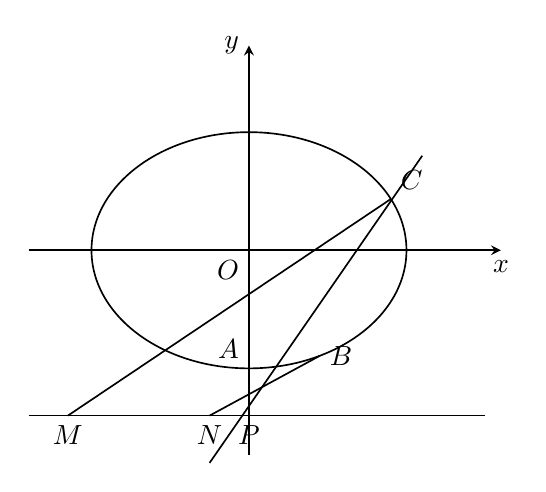
\begin{tikzpicture}[>=stealth,line width=0.6pt,font=\normalsize]
  \draw[->] (-2.8,0) -- (3.2,0) node[below] {$x$};
  \draw[->] (0,-2.6) -- (0,2.6) node[left] {$y$};
  \node[below left] at (0,0) {$O$};

  % 椭圆 x^2/5 + y^2/4 = 1, 缩放到合适大小: a=2.0, b=1.5
  \draw (0,0) ellipse (2.0 and 1.5);
  \coordinate (A) at (0,-1.5);
  \node[above left] at (A) {$A$};

  % 直线 y = -2.1 (对应 y = -3)
  \draw (-2.8,-2.1) -- (3.0,-2.1);
  \coordinate (P) at (0,-2.1);
  \node[below] at (P) {$P$};

  % 过 P 的割线交椭圆于 B, C
  \coordinate (B) at (0.9,-1.34);
  \coordinate (C) at (1.8,0.65);
  \draw (-0.5,-2.7) -- (2.2,1.2);

  % 直线 AB 交 y = -2.1 于 M, 直线 AC 交 y = -2.1 于 N
  \coordinate (M) at (-2.3,-2.1);
  \coordinate (N) at (-0.5,-2.1);

  \draw (M) -- (C);
  \draw (N) -- (B);

  \node[below] at (M) {$M$};
  \node[below] at (N) {$N$};
  \node[right] at (B) {$B$};
  \node[above right] at (C) {$C$};
\end{tikzpicture}
